\documentclass[titlepage]{article}
\usepackage[a4paper, margin=1in]{geometry}
\usepackage{graphicx} % Required for inserting images
\usepackage{amsmath}
\usepackage[style=numeric, backend=biber]{biblatex}
\addbibresource{References.bib}
\usepackage{booktabs}
\usepackage{caption}
\usepackage{multirow}
\usepackage{titling}
\usepackage{float} 


\geometry{
    a4paper,
    left=2cm,
    right=1.5cm,
    top=2cm,
    bottom=2cm,
}

\begin{document}

\begin{figure}
    \centering
    
\includegraphics[width=0.9\textwidth]{logo-86763-1.png}

\end{figure}

\title{
    \textbf{ 
        \Huge Students' Grade Performance Based on Lifestyle and Health Factors
    } 
    \vspace{20pt}
    \\
    \textbf{CS-C3240 - Machine Learning D}
    \\}

    
\date{October 2024}

\maketitle
\newpage
\section{Introduction}
\quad Machine learning has consistently demonstrated its utility and power in addressing real-world problems across a wide range of fields. When it comes to evaluating performance, particularly academic grade performance, numerous variables must be taken into account.

In this study, we will train our machine learning (ML) models using a dataset obtained from Kaggle. These models will aid both students and educators in understanding which factors most significantly influence students' grades.

Our report will begin with a Problem Formulation section, where we will clearly define the problem and outline how we intend to leverage ML models to address it. Following this, a Methods section will provide a detailed analysis of the models considered and their evaluation based on criteria such as accuracy.

In the Results section, we will present the outcomes derived from our models, followed by an in-depth analysis. Finally, the key findings will be synthesized and summarized in the Conclusion section.

\section{Problem Formulation}
\quad Our problem consists on understand how student's lifestyle and health factors affect their academic performance, so will use supervised learning models.
This study examines this problem and will try to answer and to come up with a connection between the student's lifestyle and health factors with their academic performances. We used a dataset from Kaggle \cite{Kaggle_dataset} that includes a combination of categorical and continuous variables, which influenced our choice of machine learning models.


Each datapoint represents a student and includes features related to their lifestyle. These features consist of Hours Studied, Class Attendance, Access to Resources, Previous Test Scores, Parental Involvement, and Extracurricular Activities. For our analysis, we chose to focus on features that relate more closely to lifestyle and health, specifically Parental Involvement, Extracurricular Activities, Sleep Hours, Physical Activity, and Peer Influence.

The label we selected is the Exam Score, as it provides a clear measure of academic performance. By exploring the connections between these lifestyle factors and exam scores, we hope to uncover insights into how they impact students’ educational outcomes.

\section{Methods}

\quad As our dataset contained both continuous and categorical values, the selection of machine learning (ML) methods was mainly influenced by this characteristic. With 6,607 datapoints and originally 20 columns, we decided to focus on only five key features for our problem. These features were chosen based on their direct relevance to students' health and lifestyle, which we believe they have significantly impact on the academic performance. The selected features include parental involvement, extracurricular activities, sleep hours, physical activity, and peer influence. The label for our analysis was straightforward, as it was the only one that works in our problem: the student exam scores, being a good indicator of academic performance.

The reason behind for choosing these specific features lies in their established correlation with academic outcomes. For instance, parental involvement is often linked to higher student motivation and engagement, while adequate sleep and physical activity are critical for cognitive function and overall well-being.

We were between using K-Fold Cross Validation (K-Fold) or splitting the dataset in two parts (training set and test set). As our dataset is quite large, we concluded that the best approach  would be to use K-Fold with 10 splits. We implemented this technique as it would provide more reliable and robust estimates of the model performance compared to a simple train-test split. This approach allow us to evaluate how well the model generalizes across different subsets of the data reducing the risk of overfitting. \cite{K-fold_Cross-Validation}

As we had both categorical and continuous values, we knew that our ML model choice would have to be between models that could be trained with either types of values together such as Decision Tress, Random Forest, Support Vector Classification, etc. Due to the presence of both types of values, we had to implement the LabelEnconder function from the sklearn preprocessing module, which was used to convert categorical variables into numerical format, enabling their integration in models mentioned earlier.\cite{ML_Model}

In order to choose between Random Forest Model or Decision Tress and Support Vector Classification, we decided to do some tests and carefully analyse how they differ from each other to see witch model would better suit our interests.

\subsection{Random Forest and Decision Trees}

\quad The reason why we combine Random Forest and Decision Trees models in the same subsection is easy. Basically, the Random Forest model is a combination of many decision trees. So we will now analyse the decision trees model. 

A decision tree is a supervised learning algorithm that starts with a single node (denominated by root) and splits into branches based on decisions made on each node. Basically, at each node the algorithm chooses a feature and a threshold value to split the data \cite{Randon_Forest}. In our case, it might split based on whether a student's study hours are above or below a certain number. This method is recursive and at the end, the final nodes represent the outcome. They are easy to understand and we can follow the decisions made to get to the conclusion. However, we can easily have overfitting problems, which means that we would have great accuracy for our trained data, but a really poor one on our validation set \cite{Random_Forest_Library}.

To mitigate this problem, Random Forest is often used since it predicts more accurate results, particularly when the individual trees are uncorrelated with each other. Additionally, Random Forest employs ensemble learning by averaging multiple decision trees, which helps in reducing variance and improving generalization.

\quad \textbf{Loss Functions in Decision Trees and Random Forests}

Decision Trees and Random Forests evaluate the quality of splits at each node using criteria that act as loss functions. Two primary loss functions are \textbf{Gini Impurity} and \textbf{Entropy}.

\subsubsection{Gini Impurity}

\quad \textbf{Definition:} Gini Impurity measures the probability of misclassifying a randomly chosen element based on label distribution:

\[
\text{Gini Impurity} = 1 - \sum_{i=1}^{C} p_i^2
\]

- \textbf{\( p_i \)}: Proportion of class \( i \).
- \textbf{\( C \)}: Number of classes.

\quad \textbf{Characteristics:} 
- Ranges from 0 (perfect purity) to \( 1 - \frac{1}{C} \) (maximum impurity).
- Slightly favors larger partitions and is computationally efficient.

\quad \textbf{Suitability:} Gini Impurity efficiently handles categorical variables and balances bias and variance, making it suitable for our dataset of 6,607 data points.

\subsubsection{Entropy (Information Gain)}

\quad \textbf{Definition:} Entropy quantifies the disorder in the data:

\[
\text{Entropy} = - \sum_{i=1}^{C} p_i \log_2(p_i)
\]

\quad \textbf{Characteristics:} 
- Ranges from 0 (perfect purity) to \( \log_2(C) \) (maximum entropy).
- More balanced across class distributions but slightly more computationally intensive than Gini Impurity.

\quad \textbf{Suitability:} Entropy effectively captures nuances in balanced datasets, allowing the model to identify intricate patterns in lifestyle and health factors that influence academic performance.

\quad \textbf{Comparison and Choice:} Gini Impurity is generally faster and preferred for larger datasets, while Entropy provides a detailed impurity measure beneficial for complex relationships. Depending on dataset characteristics, either can be used, with Random Forest often defaulting to Gini Impurity for efficiency.


 \subsection{Support Vector Classification - SVC}

\quad Support Vector Classification is a specialized form of the Support Vector Machine, designed specifically for classification tasks. The model works by distinguishing between two classes through the identification of an optimal hyperplane that maximizes the margin between the closest data points from opposing classes \cite{SVM}.

SVM is valuable due to its ability to manage non-linear relationships using the kernel trick, which reconfigures input data into a higher-dimensional space where linear separation becomes possible. In essence, the algorithm searches for the best hyperplane to separate the two classes while maximizing the margin. Once the support vectors—the points closest to the hyperplane—are identified, the model calculates the hyperplane by maximizing the distance between it and the support vectors. After establishing the hyperplane, new data points are classified based on which side of the boundary they fall.

A major strength of this model is its versatility. The kernel trick allows it to handle non-linear decision boundaries, making it particularly effective when the number of features exceeds the number of data points. However, SVM's performance tends to decline as dataset size increases, and selecting the right kernel and tuning parameters (\( C \) and \( \gamma \)) can be difficult, often requiring cross-validation for optimization.

\quad \textbf{Loss Functions in Support Vector Classification (SVC)}

Support Vector Classification relies on specific loss functions to optimize the decision boundary. Two prominent loss functions are \textbf{Hinge Loss} and \textbf{Squared Hinge Loss}.

\subsubsection{Hinge Loss}

\quad \textbf{Definition:} Hinge Loss is defined as:

\[
\text{Hinge Loss} = \max(0, 1 - y_i \cdot f(x_i))
\]

- \textbf{\( y_i \)}: True label of the \(i\)-th sample (\(+1\) or \(-1\)).
- \textbf{\( f(x_i) \)}: Decision function output for the \(i\)-th sample.

\quad \textbf{Characteristics:} 
- Promotes margin maximization, requiring correct classifications with a margin of at least 1.
- Less sensitive to outliers by assigning zero loss to correctly classified points beyond the margin.
- The convexity of Hinge Loss ensures efficient optimization.

\quad \textbf{Suitability:} This loss function effectively balances correct classification with margin maximization, leading to a more generalizable model for predicting student performance based on lifestyle and health factors.

\subsubsection{Squared Hinge Loss}

\quad \textbf{Definition:} Squared Hinge Loss is:

\[
\text{Squared Hinge Loss} = \max(0, 1 - y_i \cdot f(x_i))^2
\]

\quad \textbf{Characteristics:} 
- Increases penalties for misclassifications by squaring the margin violation.
- Provides a smoother loss function for gradient-based optimizations.
- Encourages larger margins compared to standard Hinge Loss.

\quad \textbf{Suitability:} This loss function is useful for scenarios requiring stricter penalties for misclassifications, enhancing the model's robustness and ability to generalize in predicting academic performance.

\quad \textbf{Comparison:} While both loss functions aim to maximize the margin, Squared Hinge Loss introduces a steeper penalty for misclassified points within the margin, making it beneficial when reducing errors is critical. The choice between the two depends on the problem's specific needs, with Squared Hinge Loss preferred for stricter classification boundaries.


\section{Results}

\subsection{ML Model Decision}

In this section, we evaluate the performance of the machine learning models employed in our analysis, specifically focusing on Random Forest and Support Vector Classification (SVC). The training accuracy for the Random Forest model was 91.91\%, while the SVC achieved a slightly higher training accuracy of 94.49\%. Similarly, during validation, the Random Forest model produced an accuracy of 90.87\%, compared to 94.41\% for SVC. 

The results indicate that while both models performed well, SVC exhibited superior accuracy in both training and validation phases. This suggests that SVC may be better suited for the dataset at hand, particularly in distinguishing between the classes with a more nuanced decision boundary.

Therefore, the final choosen method is SVC.

A key factor in the performance of Support Vector Classification (SVC) is the hinge loss function, which is crucial for optimizing the model. Hinge loss, primarily used in SVM models, is defined as follows \cite{Hinge-loss}:

\begin{equation}
\text{Hinge Loss} = \max(0, 1 - y_i \cdot f(x_i))
\end{equation}

In this equation, \(y_i\) represents the true label of the data point, and \(f(x_i)\) is the model's output for that data point. Hinge loss penalizes misclassifications and encourages correct classifications to occur with a margin. Specifically, the loss is zero when the prediction is correct and lies beyond the margin (i.e., \(y_i \cdot f(x_i) > 1\)). However, if a prediction falls within the margin or is incorrect, the loss increases, prompting adjustments in the model \cite{Predicting_Wine_Quality}.

We chose hinge loss for our SVC model because it not only focuses on correctly classifying data points but also emphasizes maximizing the margin between classes. This characteristic is particularly advantageous in our context, as it enhances the model’s robustness and generalization capability. Given the results of our model comparison (Fig \ref{fig:enter-label}), it appears that SVC's effective utilization of hinge loss, in conjunction with the kernel trick for managing non-linear relationships, provides a significant advantage over Random Forest. This allows SVC to perform better in accurately predicting student academic performance based on lifestyle and health factors.

\begin{figure}[H]
    \centering
    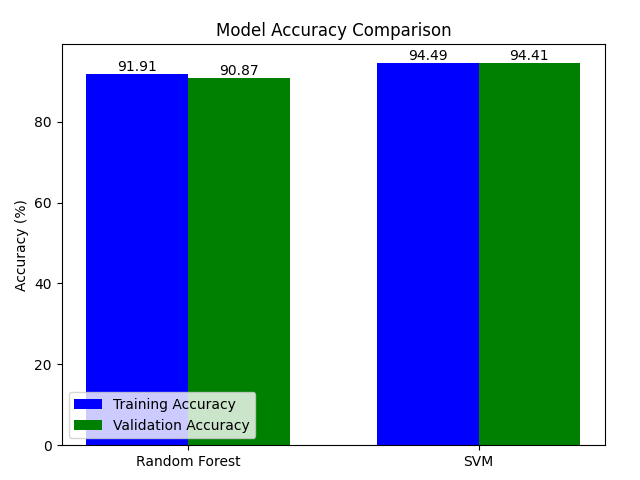
\includegraphics[width=0.5\linewidth]{Figure_1.png}
    \caption{Model Accuracy Comparison}
    \label{fig:enter-label}
\end{figure}

\subsection{Performance Measurement Indicators}

In this project, where the goal is to predict numerical grades between 0 and 100, it is more appropriate to use evaluation metrics such as Mean Absolute Error (MAE), Mean Squared Error (MSE), Root Mean Squared Error (RMSE), and R-squared (R²) instead of accuracy, precision, recall, and F1-score. The reason behind this choice lies in the nature of the prediction task. Accuracy, precision, recall, and F1-score are metrics designed primarily for classification problems, where the outcomes are discrete categories. In contrast, our task involves continuous numerical predictions, making it essential to evaluate how closely our predicted values align with the actual grades.

\subsection{Data-Driven Results}

In this project, three machine learning models—SVR, DecisionTree, and RandomForest—were evaluated using four primary metrics: Mean Absolute Error (MAE), Mean Squared Error (MSE), Root Mean Squared Error (RMSE), and R-squared (R²). These metrics were used to assess both training and validation performance across all cross-validation folds.

\begin{table}[!ht]
    \centering
    \caption{\textbf{Model Performance Comparison Across Sets}}
    \renewcommand{\arraystretch}{1.3} % Adjust spacing factor
    \scriptsize % Adjust font size
    \setlength{\tabcolsep}{4pt} % Adjust column padding
    \label{table:comparison_models}
    \begin{tabular}{l cccc cccc cccc }
        \toprule
        \multirow{2}{*}{\textbf{Method}} & \multicolumn{4}{c}{\textbf{Training Set}} & \multicolumn{4}{c}{\textbf{Validation Set}} & \multicolumn{4}{c}{\textbf{Test Set}} \\
        \cmidrule(lr){2-5} \cmidrule(lr){6-9} \cmidrule(lr){10-13}
        & \textbf{MAE} & \textbf{MSE} & \textbf{RMSE} & \textbf{R²} 
        & \textbf{MAE} & \textbf{MSE} & \textbf{RMSE} & \textbf{R²} 
        & \textbf{MAE} & \textbf{MSE} & \textbf{RMSE} & \textbf{R²} \\
        \midrule
        SVR & 2.8130 & 15.0286 & 3.8766 & 0.0229 
            & 2.8184 & 15.0588 & 3.8722 & 0.0190 
            & 2.7958 & 13.9780 & 3.7387 & 0.0111 \\
        Decision Tree & 2.6016 & 12.9563 & 3.5994 & 0.1576 
                     & 2.9984 & 17.1152 & 4.1313 & -0.1215 
                     & -- & -- & -- & -- \\
        Random Forest & 2.6329 & 13.0307 & 3.6097 & 0.1528 
                     & 2.9740 & 16.6861 & 4.0788 & -0.0916 
                     & -- & -- & -- & -- \\
        \bottomrule
    \end{tabular}
\end{table}






\section{Conclusion}
The analysis of the models reveals that while SVR showed the most consistent performance, the results, particularly the low R² scores across all models, indicate that the models were unable to capture the underlying variance in the data. The low discrepancy between training and validation errors suggests minimal overfitting, yet the overall performance could be improved. None of the models seem to have achieved optimal results, as indicated by the relatively low R² scores and moderate error rates.

To further improve the results, several strategies can be considered. First, incorporating additional or more relevant features may help better explain the variance in student performance. Exploring more sophisticated models or ensemble methods, such as Gradient Boosting or tuning hyperparameters more thoroughly, could also improve predictions. Additionally, experimenting with different loss functions tailored to the specific distribution of the data might result in better accuracy. Finally, increasing the size of the training dataset or refining data preprocessing steps could also yield more robust results in future work.



\newpage
\printbibliography

\section{Appendix}

The link for the repository: \url{https://github.com/guilhermecruz760/Aalto-Machine-Learning-Project}



\end{document}
